% ============================================================================
% CHƯƠNG 1: GIỚI THIỆU VỀ LẬP TRÌNH SONG SONG
% ============================================================================
\chapter{Giới thiệu về Lập trình Song song}
\label{chap:introduction}

\section{Đặt vấn đề}

Trong những thập kỷ qua, sự phát triển của khoa học máy tính đã chứng kiến những bước tiến vượt bậc về khả năng tính toán. Tuy nhiên, với sự bùng nổ của dữ liệu lớn (Big Data), trí tuệ nhân tạo (AI), học máy (Machine Learning) và học sâu (Deep Learning), nhu cầu về sức mạnh tính toán ngày càng tăng cao, vượt xa khả năng của các bộ xử lý đơn lõi truyền thống.

\textbf{Định luật Moore} - dự đoán rằng số lượng transistor trên một chip sẽ tăng gấp đôi sau mỗi 18-24 tháng - đang dần đạt đến giới hạn vật lý. Thay vì tiếp tục tăng tốc độ xung nhịp của một lõi đơn, các nhà sản xuất chip đã chuyển hướng sang phát triển các bộ xử lý đa lõi (multi-core) và mảng xử lý song song (parallel processing arrays).

\begin{figure}[H]
\centering
\begin{tikzpicture}[scale=0.9]
    % Timeline
    \draw[thick,->] (0,0) -- (14,0) node[right] {Thời gian};
    
    % Era markers
    \foreach \x/\year in {1/1970, 3/1980, 5/1990, 7/2000, 9/2010, 11/2020, 13/2025} {
        \draw (\x,0.1) -- (\x,-0.1) node[below] {\tiny\year};
    }
    
    % CPU frequency curve
    \draw[thick,blue,smooth] plot coordinates {
        (1,0.5) (3,1) (5,1.8) (7,3) (8.5,4) (9,4.2) (11,4.3) (13,4.4)
    };
    \node[blue,above] at (7,3.2) {\footnotesize CPU Frequency};
    
    % Parallel cores curve
    \draw[thick,red,smooth,dashed] plot coordinates {
        (7,0.5) (9,1.5) (11,3.5) (13,5)
    };
    \node[red,above] at (11,4) {\footnotesize \# Cores};
    
    % GPU compute power curve
    \draw[thick,cudagreen,smooth,dotted,very thick] plot coordinates {
        (7,0.3) (9,2) (11,4) (13,6)
    };
    \node[cudagreen,above] at (13,6.2) {\footnotesize GPU Power};
    
    % Vertical line at frequency wall
    \draw[gray,dashed] (9,0) -- (9,5) node[above,font=\tiny] {Bức tường tần số};
\end{tikzpicture}
\caption{Xu hướng phát triển: từ tăng tần số sang đa lõi và GPU}
\label{fig:trend}
\end{figure}

\section{Lập trình Tuần tự vs Song song}

\subsection{Lập trình Tuần tự (Sequential Programming)}

Trong mô hình lập trình tuần tự truyền thống, các chỉ thị (instructions) được thực thi \textbf{lần lượt}, cái này hoàn thành rồi mới đến cái tiếp theo. CPU với kiến trúc Von Neumann được tối ưu hóa cho:
\begin{itemize}
    \item \textbf{Độ trễ thấp (Low latency)}: Hoàn thành một tác vụ nhanh nhất có thể
    \item \textbf{Xử lý logic phức tạp}: Branch prediction, out-of-order execution
    \item \textbf{Cache lớn}: Giảm thời gian truy cập bộ nhớ
\end{itemize}

\begin{lstlisting}[caption={Ví dụ: Cộng hai vector tuần tự trên CPU}, label={lst:seq_sum}]
void sumHost(float *a, float *b, float *c, int n) {
    for (int i = 0; i < n; i++) {
        c[i] = a[i] + b[i];  // Thuc hien tuan tu tung phan tu
    }
}
\end{lstlisting}

\subsection{Lập trình Song song (Parallel Programming)}

Lập trình song song chia bài toán lớn thành nhiều tác vụ nhỏ và thực thi \textbf{đồng thời} trên nhiều bộ xử lý. GPU với hàng nghìn lõi nhỏ được tối ưu hóa cho:
\begin{itemize}
    \item \textbf{Băng thông cao (High throughput)}: Xử lý nhiều dữ liệu cùng lúc
    \item \textbf{Tính toán song song khối lượng lớn}: Hàng triệu thread cùng hoạt động
    \item \textbf{Hiệu quả năng lượng}: FLOPS/Watt cao hơn CPU
\end{itemize}

\begin{figure}[H]
\centering
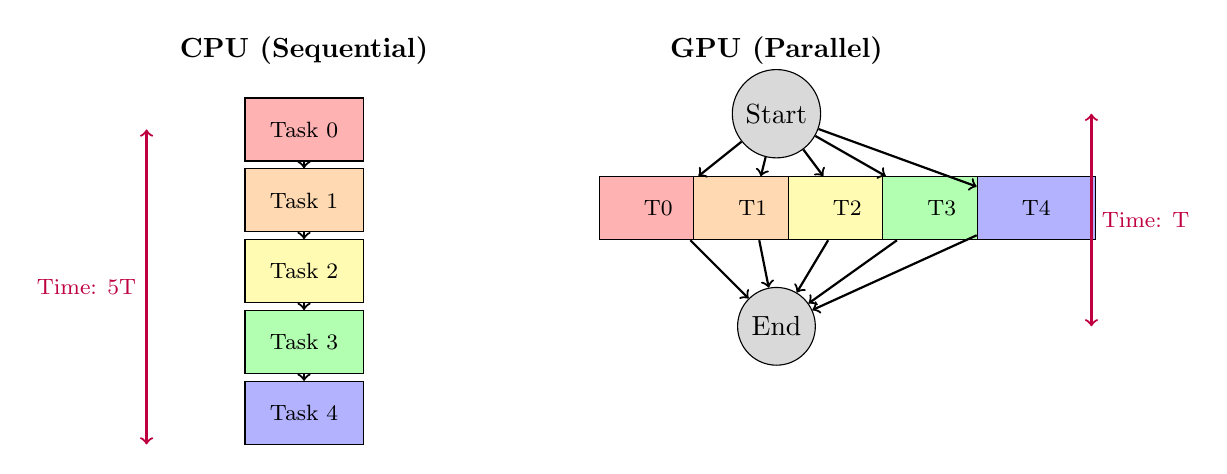
\begin{tikzpicture}[
    box/.style={draw, minimum width=1.5cm, minimum height=0.8cm, font=\footnotesize},
    arrow/.style={->, thick}
]
    % CPU side
    \node[font=\bfseries] at (-3,3) {CPU (Sequential)};
    
    % Sequential boxes
    \foreach \i/\c in {0/red!30, 1/orange!30, 2/yellow!30, 3/green!30, 4/blue!30} {
        \node[box, fill=\c] (seq\i) at (-3, 2-\i*0.9) {Task \i};
    }
    \foreach \i in {0,...,3} {
        \pgfmathtruncatemacro{\j}{\i+1}
        \draw[arrow] (seq\i) -- (seq\j);
    }
    
    % GPU side
    \node[font=\bfseries] at (3,3) {GPU (Parallel)};
    
    % Parallel boxes
    \foreach \i/\c in {0/red!30, 1/orange!30, 2/yellow!30, 3/green!30, 4/blue!30} {
        \node[box, fill=\c] (par\i) at ({1.5+\i*1.2}, 1) {T\i};
    }
    
    % Start and end points
    \node[draw, circle, fill=gray!30] (start) at (3,2.2) {Start};
    \node[draw, circle, fill=gray!30] (end) at (3,-0.5) {End};
    
    \foreach \i in {0,...,4} {
        \draw[arrow] (start) -- (par\i);
        \draw[arrow] (par\i) -- (end);
    }
    
    % Time arrows
    \draw[<->,thick,purple] (-5,2) -- (-5,-2) node[midway,left,font=\footnotesize] {Time: 5T};
    \draw[<->,thick,purple] (7,2.2) -- (7,-0.5) node[midway,right,font=\footnotesize] {Time: T};
    
\end{tikzpicture}
\caption{So sánh thực thi tuần tự và song song}
\label{fig:seq_vs_par}
\end{figure}

\section{Giới thiệu về CUDA}

\subsection{CUDA là gì?}

\textbf{CUDA} (Compute Unified Device Architecture) là nền tảng tính toán song song và mô hình lập trình được phát triển bởi NVIDIA từ năm 2006. CUDA cho phép các lập trình viên sử dụng ngôn ngữ cấp cao (C, C++, Fortran, Python) để khai thác sức mạnh tính toán của GPU cho các mục đích tính toán tổng quát (GPGPU - General-Purpose computing on GPU).

\begin{table}[H]
\centering
\caption{So sánh CPU và GPU}
\label{tab:cpu_vs_gpu}
\begin{tabular}{@{}lcc@{}}
\toprule
\textbf{Đặc điểm} & \textbf{CPU} & \textbf{GPU} \\
\midrule
Số lõi & 4 - 64 & 1,000 - 10,000+ \\
Tốc độ xung nhịp & 3 - 5 GHz & 1 - 2 GHz \\
Cache & Lớn (MB) & Nhỏ (KB/core) \\
Kiểu tính toán & Low latency & High throughput \\
Tối ưu cho & Logic phức tạp & Tính toán lặp lại \\
Ví dụ & Intel Core i9 & NVIDIA Tesla T4 \\
\bottomrule
\end{tabular}
\end{table}

\subsection{Mô hình lập trình CUDA}

Chương trình CUDA bao gồm hai phần chính:
\begin{enumerate}
    \item \textbf{Host code}: Chạy trên CPU, quản lý bộ nhớ, điều khiển luồng thực thi
    \item \textbf{Device code}: Chạy trên GPU, thực hiện tính toán song song (kernel functions)
\end{enumerate}

\begin{figure}[H]
\centering
\begin{tikzpicture}[
    hostbox/.style={draw, fill=blue!10, rounded corners, minimum width=4cm, minimum height=1cm},
    devbox/.style={draw, fill=green!10, rounded corners, minimum width=4cm, minimum height=1cm},
    arrow/.style={->, thick, >=stealth}
]
    % Host side
    \node[font=\bfseries\large, blue] at (-3, 4) {HOST (CPU)};
    \node[hostbox] (h1) at (-3, 3) {Khởi tạo dữ liệu};
    \node[hostbox] (h2) at (-3, 1.8) {cudaMalloc()};
    \node[hostbox] (h3) at (-3, 0.6) {cudaMemcpy() H2D};
    \node[hostbox] (h4) at (-3, -0.6) {Kernel<<<>>>()};
    \node[hostbox] (h5) at (-3, -1.8) {cudaMemcpy() D2H};
    \node[hostbox] (h6) at (-3, -3) {cudaFree()};
    
    % Device side
    \node[font=\bfseries\large, green!50!black] at (3, 4) {DEVICE (GPU)};
    \node[devbox] (d1) at (3, 1.8) {Cấp phát VRAM};
    \node[devbox] (d2) at (3, 0.6) {Nhận dữ liệu};
    \node[devbox, minimum height=1.5cm] (d3) at (3, -0.9) {Thực thi Kernel\\(Hàng nghìn threads)};
    \node[devbox] (d4) at (3, -2.4) {Trả kết quả};
    
    % Arrows
    \draw[arrow] (h1) -- (h2);
    \draw[arrow] (h2) -- (h3);
    \draw[arrow] (h3) -- (h4);
    \draw[arrow] (h4) -- (h5);
    \draw[arrow] (h5) -- (h6);
    
    \draw[arrow,dashed,blue] (h2) -- (d1);
    \draw[arrow,dashed,red] (h3) -- (d2);
    \draw[arrow,dashed,green!50!black,very thick] (h4) -- (d3);
    \draw[arrow,dashed,red] (d3) -- (h5);
    
\end{tikzpicture}
\caption{Luồng thực thi của chương trình CUDA}
\label{fig:cuda_flow}
\end{figure}

\subsection{Kernel Function}

Kernel là hàm đặc biệt chạy trên GPU, được đánh dấu bằng từ khóa \code{\_\_global\_\_}. Khi gọi kernel, ta chỉ định số lượng thread thông qua cú pháp \code{<<<grid, block>>>}.

\begin{lstlisting}[caption={Cấu trúc cơ bản của một CUDA kernel}, label={lst:kernel_basic}]
// Dinh nghia kernel - chay tren GPU
__global__ void myKernel(float *data, int n) {
    // Tinh chi so global cua thread
    int idx = blockIdx.x * blockDim.x + threadIdx.x;
    
    // Kiem tra bien (Boundary check)
    if (idx < n) {
        data[idx] = data[idx] * 2.0f;  // Xu ly du lieu
    }
}

// Goi kernel tu Host
int main() {
    // ... cap phat bo nho ...
    
    dim3 block(256);                         // 256 threads/block
    dim3 grid((n + block.x - 1) / block.x);  // So block can thiet
    
    myKernel<<<grid, block>>>(d_data, n);    // Goi kernel
    cudaDeviceSynchronize();                 // Cho GPU hoan thanh
    
    // ... copy ket qua ve ...
}
\end{lstlisting}

\section{Thiết lập môi trường}

\subsection{Yêu cầu hệ thống}

Để phát triển ứng dụng CUDA, cần có:
\begin{itemize}
    \item \textbf{Phần cứng}: GPU NVIDIA hỗ trợ kiến trúc CUDA (từ Compute Capability 3.0 trở lên)
    \item \textbf{Phần mềm}: NVIDIA Driver và CUDA Toolkit tương thích
\end{itemize}

\subsection{Google Colab - Giải pháp đám mây miễn phí}

Đối với sinh viên không có GPU NVIDIA, \textbf{Google Colab} là giải pháp lý tưởng:

\begin{enumerate}
    \item Truy cập \url{https://colab.research.google.com}
    \item Tạo notebook mới
    \item Chọn \textbf{Runtime $\rightarrow$ Change runtime type $\rightarrow$ GPU}
    \item Sử dụng plugin \code{nvcc4jupyter} để biên dịch code CUDA
\end{enumerate}

\begin{lstlisting}[language=Python, caption={Cài đặt và sử dụng CUDA trên Google Colab}]
# Kiem tra GPU
!nvidia-smi

# Cai dat plugin nvcc4jupyter
!pip install nvcc4jupyter
%load_ext nvcc4jupyter

# Viet code CUDA trong cell
%%cuda
#include <stdio.h>

__global__ void hello() {
    printf("Hello from GPU thread %d!\n", threadIdx.x);
}

int main() {
    hello<<<1, 10>>>();
    cudaDeviceSynchronize();
    return 0;
}
\end{lstlisting}

\section{Kết luận chương}

Chương này đã giới thiệu các khái niệm nền tảng về lập trình song song và CUDA:

\begin{itemize}
    \item \textbf{Nhu cầu song song hóa}: Do giới hạn vật lý của CPU đơn lõi, song song hóa là xu hướng tất yếu
    \item \textbf{GPU vs CPU}: GPU tối ưu cho throughput, CPU tối ưu cho latency
    \item \textbf{CUDA}: Nền tảng mạnh mẽ để khai thác GPU NVIDIA cho tính toán khoa học
    \item \textbf{Google Colab}: Giải pháp tiếp cận GPU miễn phí cho sinh viên
\end{itemize}

Các chương tiếp theo sẽ đi sâu vào mô hình lập trình CUDA và các thuật toán song song cụ thể.
